\chapter{高频电外科发生器系统硬件设计}

\section{引言}

\section{电源模块设计}
本文所设计的高频电外科发生器系统的电源模块主要用于为系统各功能模块提供稳定、可靠的供电电源，其结构主要由医疗级开关电源模块与板载低压辅助电源管理电路两部分构成，如图\ref{system}所示。系统输入电源为220V交流市电，首先经医疗级开关电源模块完成初级的的交流-直流（AC/DC）变换得到稳定的直流输出电压。其中，一路直流电压直接作为高频能量发生主电路的输入电源，其余直流电压经板载低压辅助电源管理电路进行滤波、降压与稳压处理后，生成不同电压等级的辅助电源，用于供给系统中的控制模块、人机交互模块等低压功能模块使用。

\subsection{医疗级开关电源选型}
在本系统中，电源模块负责为整机提供稳定的能量来源，对于操作者和患者的电气安全至关重要，因此本文优先选用独立的医疗电源模块对输入电源进行变换处理。医疗电源是专门面向医疗设备应用场景设计的AC/DC或DC/DC电源模块，能够在复杂的电磁环境下安全稳定、低噪声地供电。医疗电源在设计和制造过程中需严格遵循医疗类安规认证（IEC-60601）并通过复杂的电磁干扰与兼容性测试，相较于普通工业级电源，其在输入输出侧通常采用双重或加强绝缘结构（MOPP），耐压等级可达4KV以上，同时将漏电流严格控制在微安级别，有效降低了手术过程中因寄生电容耦合或共模干扰引起的安全风险。

目前市场上医疗电源产品较为成熟，常见的厂商有明纬、台达以及金升阳等。在具体选型过程中需结合系统整体设计指标与功能需求，从以下两个方面进行重点考量：一方面，系统最大输出功率需达到 100 W，考虑到高频能量发生主电路存在的转换损耗与其他功能模块的功率消耗，所选医疗电源模块应具备充足的功率裕量；另一方面，系统采用直流调功方式控制高频输出功率，因此医疗电源模块向可调降压稳压电路提供的直流输出电压需达到一定幅值，以保证系统具备足够的功率调节范围。

基于上述分析，本文选用明纬公司生产的RPS-300-48和RPT-60B两组医疗级电源模块。其中前者用于为高频能量发生主电路提供48V直流电源，后者则用于为系统低压辅助电源管理电路提供多路低压输出。两组医疗电源模块的主要工作参数如表\ref{medical_power}所示。

\begin{table}[htbp]
    \caption{\label{medical_power}医疗级开关电源主要工作参数}
    \centering
    \small
    \setlength{\tabcolsep}{20pt}
	\begin{tabular}{ c c c }
        \hline
        参数 & RPS-300-48 & RPT-60B\\
        \hline
        输出电压            &  48V  & ±12V/5V\\
        输出功率（自然风冷）            &  200W & 50W\\
        电压精度            &  ±2.0\%  & ±3.0\% / ±6.0\%\\ 
        效率               &  93\%  & 78\%\\
        \hline
    \end{tabular}
\end{table}

\subsection{低压辅助电源设计}
在本文所设计的的电源系统中，低压辅助电源需要给控制单元芯片、继电器、运算放大器、功率器件驱动电路、隔离电路以及采样电路等进行优质可靠供电。根据系统芯片的供电需求，辅助电源需提供+12V、-12V、5V和3.3V四种不同电压等级的低压电源。同时，为降低高频输出信号对控制系统的干扰，并满足电外科发生器的安全要求，系统还需为隔离区模块及外设检测电路提供独立的隔离电源。

\begin{figure}[htbp]
\centering
\begin{minipage}[c]{0.5\textwidth}
\centering
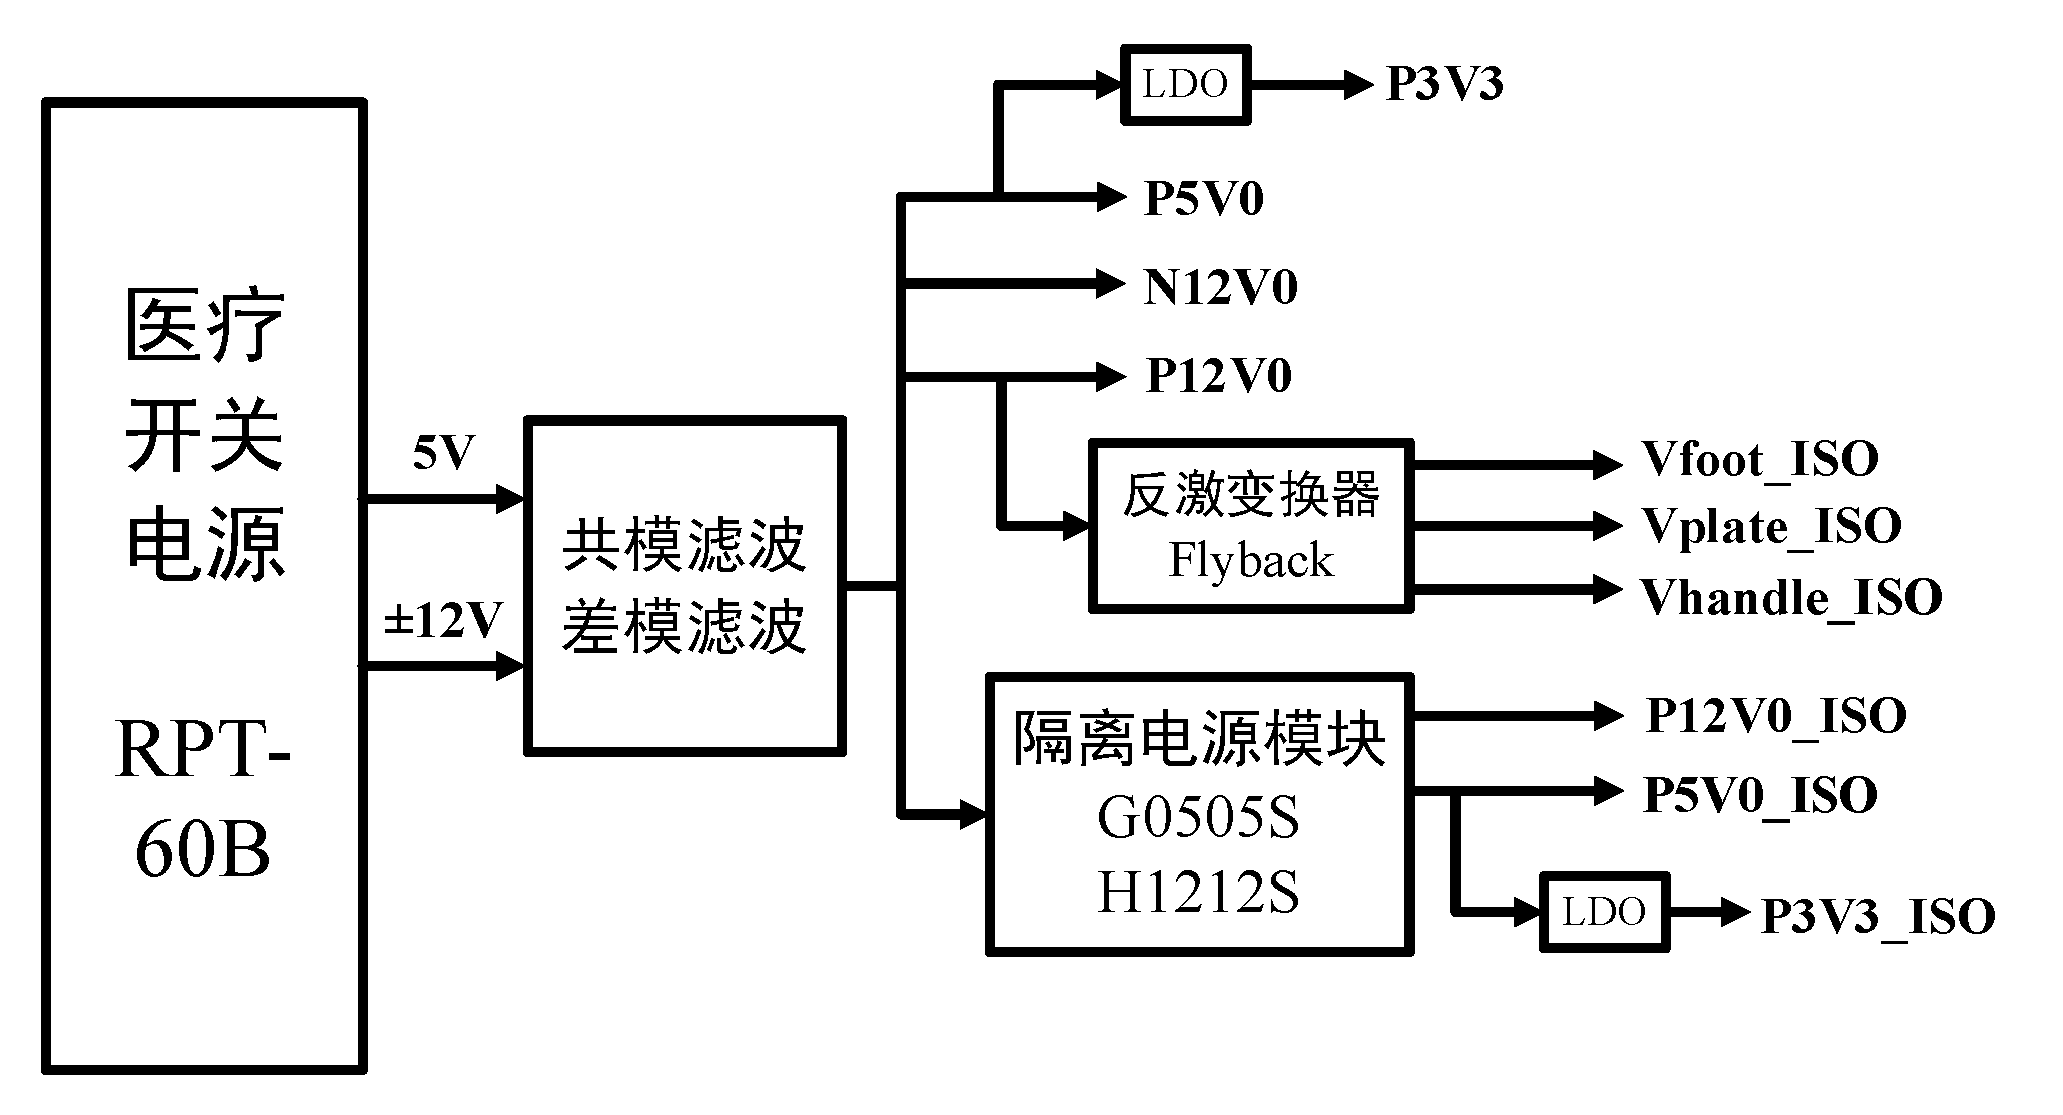
\includegraphics[scale=0.24]{Fig/power_structure.pdf} %1:1导入
\end{minipage}%
\begin{minipage}[c]{0.5\textwidth}
\centering
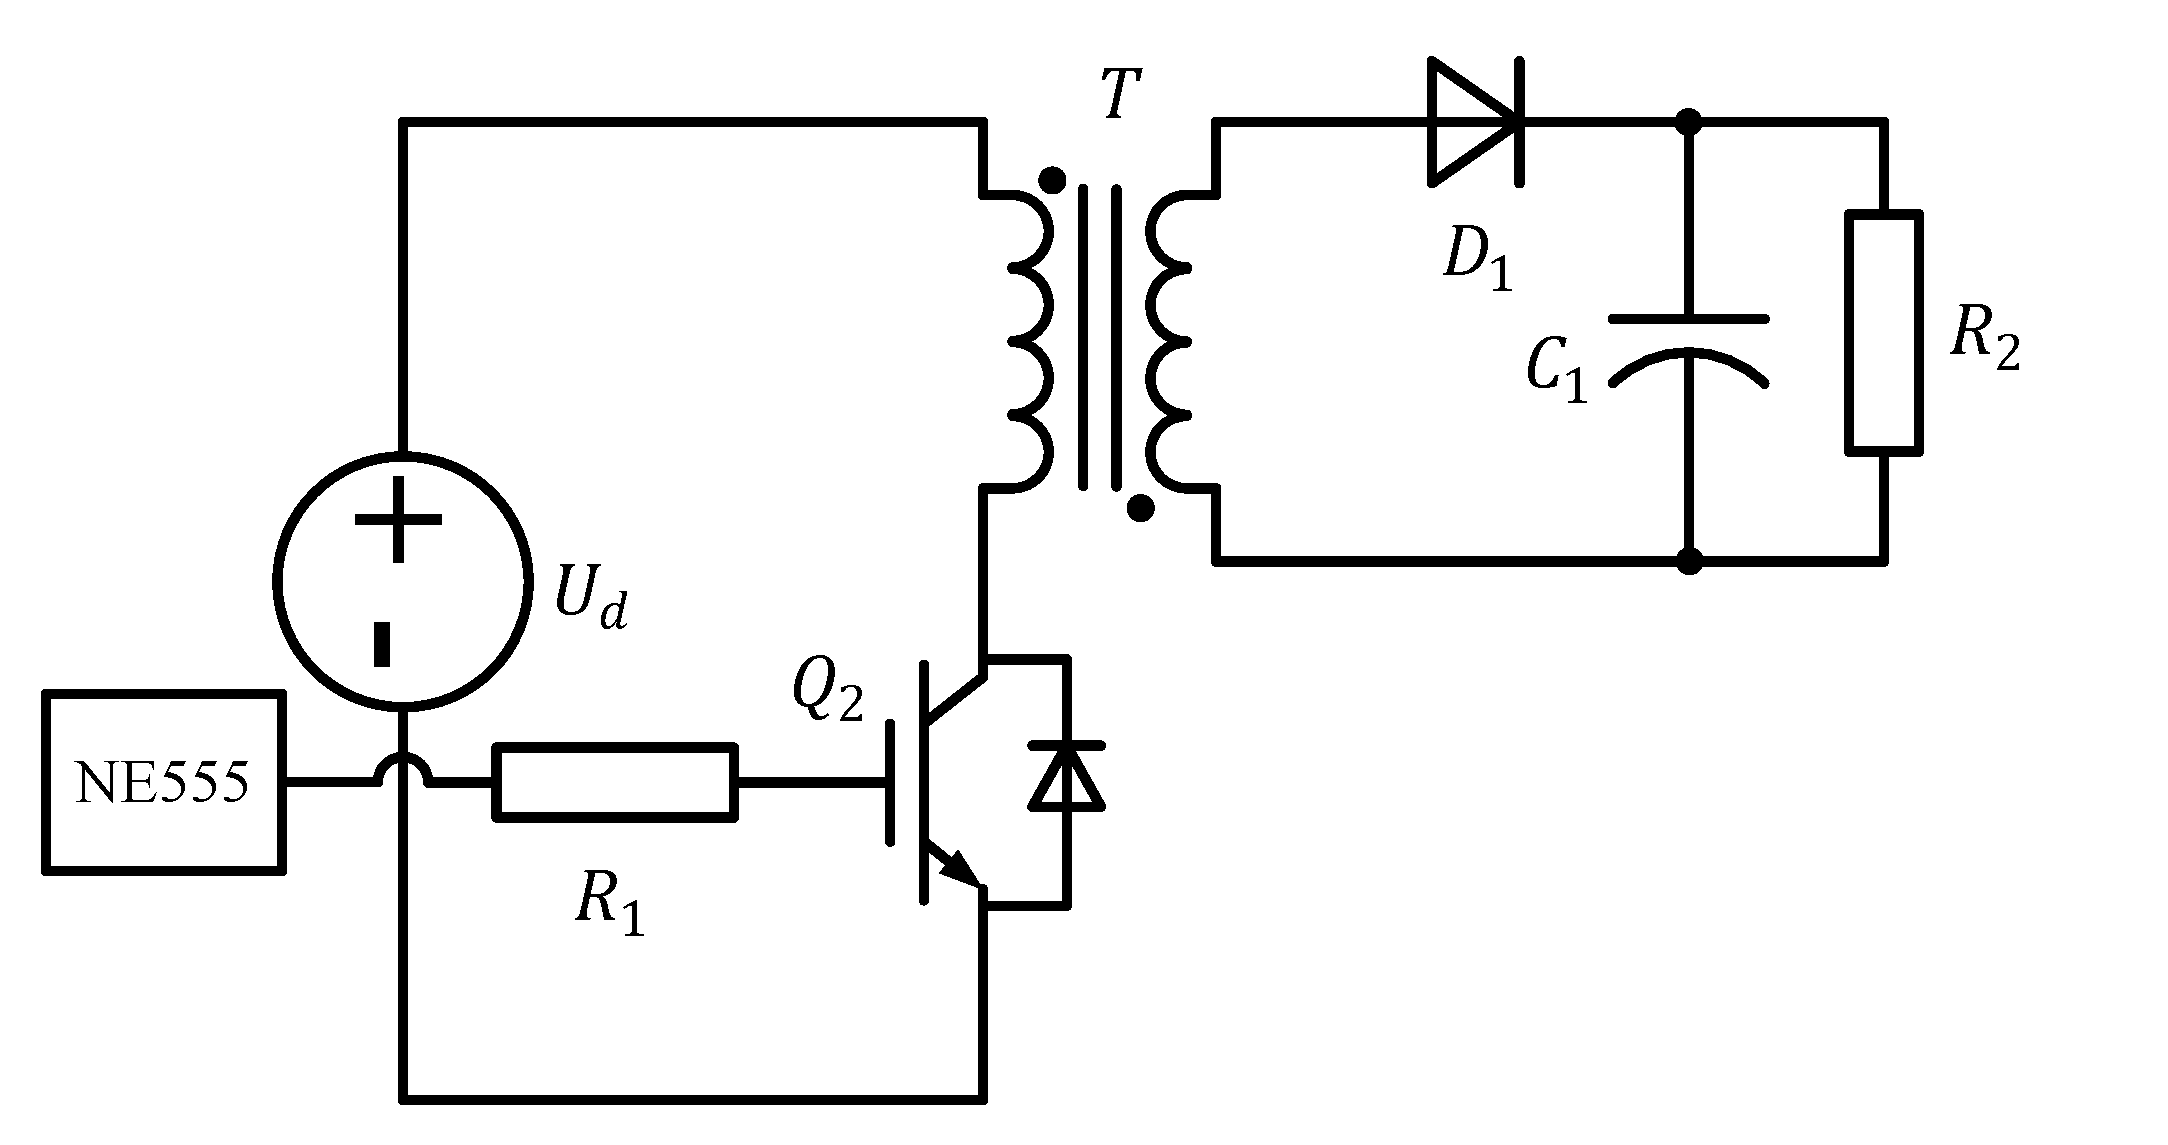
\includegraphics[scale=0.23]{Fig/Flyback.pdf}
\end{minipage}\\[1pt]
\begin{minipage}[t]{0.5\textwidth} % 以下为新添加页面划分，[t]表示行顶部对齐
\caption{\label{power_structure}低压辅助电源架构}
\end{minipage}%
\begin{minipage}[t]{0.5\textwidth}
\caption{\label{Flyback}反激变换器拓扑结构}
\end{minipage}%
\end{figure}

本设计方案中低压辅助电源架构如图\ref{power_structure}所示，医疗级开关电源模块RPT-60B输出±12V、5V电源首先经过共模与差模滤波电路，以抑制开关噪声及电源纹波。对于非隔离区供电部分，采用线性稳压器（LDO）SPX1117由5V电源进一步生成3.3V电源，为 MCU 及低噪声敏感的数字控制电路提供稳定供电；对于隔离区供电部分，则采用隔离电源模块H0505S和H1212S，分别生成±5V和12V的隔离直流电源，其中5V隔离电源经线性稳压器进一步转换为3.3V隔离电源，用于为隔离区的主控处理器和采样通信电路稳定供电，从而实现控制侧与功率输出侧之间的电气隔离。

此外，针对手柄、脚踏及中性极板等外设接口电路，本文采用反激式（Flyback）变换器实现隔离供电，其工作原理如图\ref{Flyback}所示。反激变换器中，功率MOS管由占空比为50\% ，频率为250KHz的方波驱动信号控制，当开关管导通时，变压器原边电感电流上升，由于原副边极性关系，副边整流二极管处于截止状态，能量以磁能形式储存在变压器中，负载由输出滤波电容提供能量；当开关管关断时，变压器原边电感感应电压极性反转，副边整流二极管导通，变压器储存的能量经二极管向负载释放，同时对输出电容充电，从而实现隔离供电。


\section{高频能量发生模块设计}
在电源模块提供的直流源基础上，为了实现高频、大功率信号的发生与输出功率的可调，系统通过高频能量发生模块完成直流-交流（DC/AC）变换、信号放大与功率调节等功能，其电路拓扑包含可调降压稳压直流源-推挽逆变电路-LC谐振网络三级结构。
\subsection{可调式直流稳压源}
可调式直流降压稳压电路本质上是一种可调节输出电压的Buck降压变换器，其输入为电源模块提供的48V输入电源，输出为可调节范围为2.5V-48V的直流电压，通过调整反馈引脚处的偏置电压来调节输出的直流电压值。本文选择使用降压型稳压芯片LT1074HV为核心器件构建可调直流稳压源电路如图\ref{buck_adjust}所示，其中LT1074构成可调降压稳压电路，TLC5615数模转换芯片与LM358运算放大器构成偏置电压调节电路。

\begin{figure}[htbp]
% 该图片比例为多次调试过后的最大值，再大就要溢出了
\centering
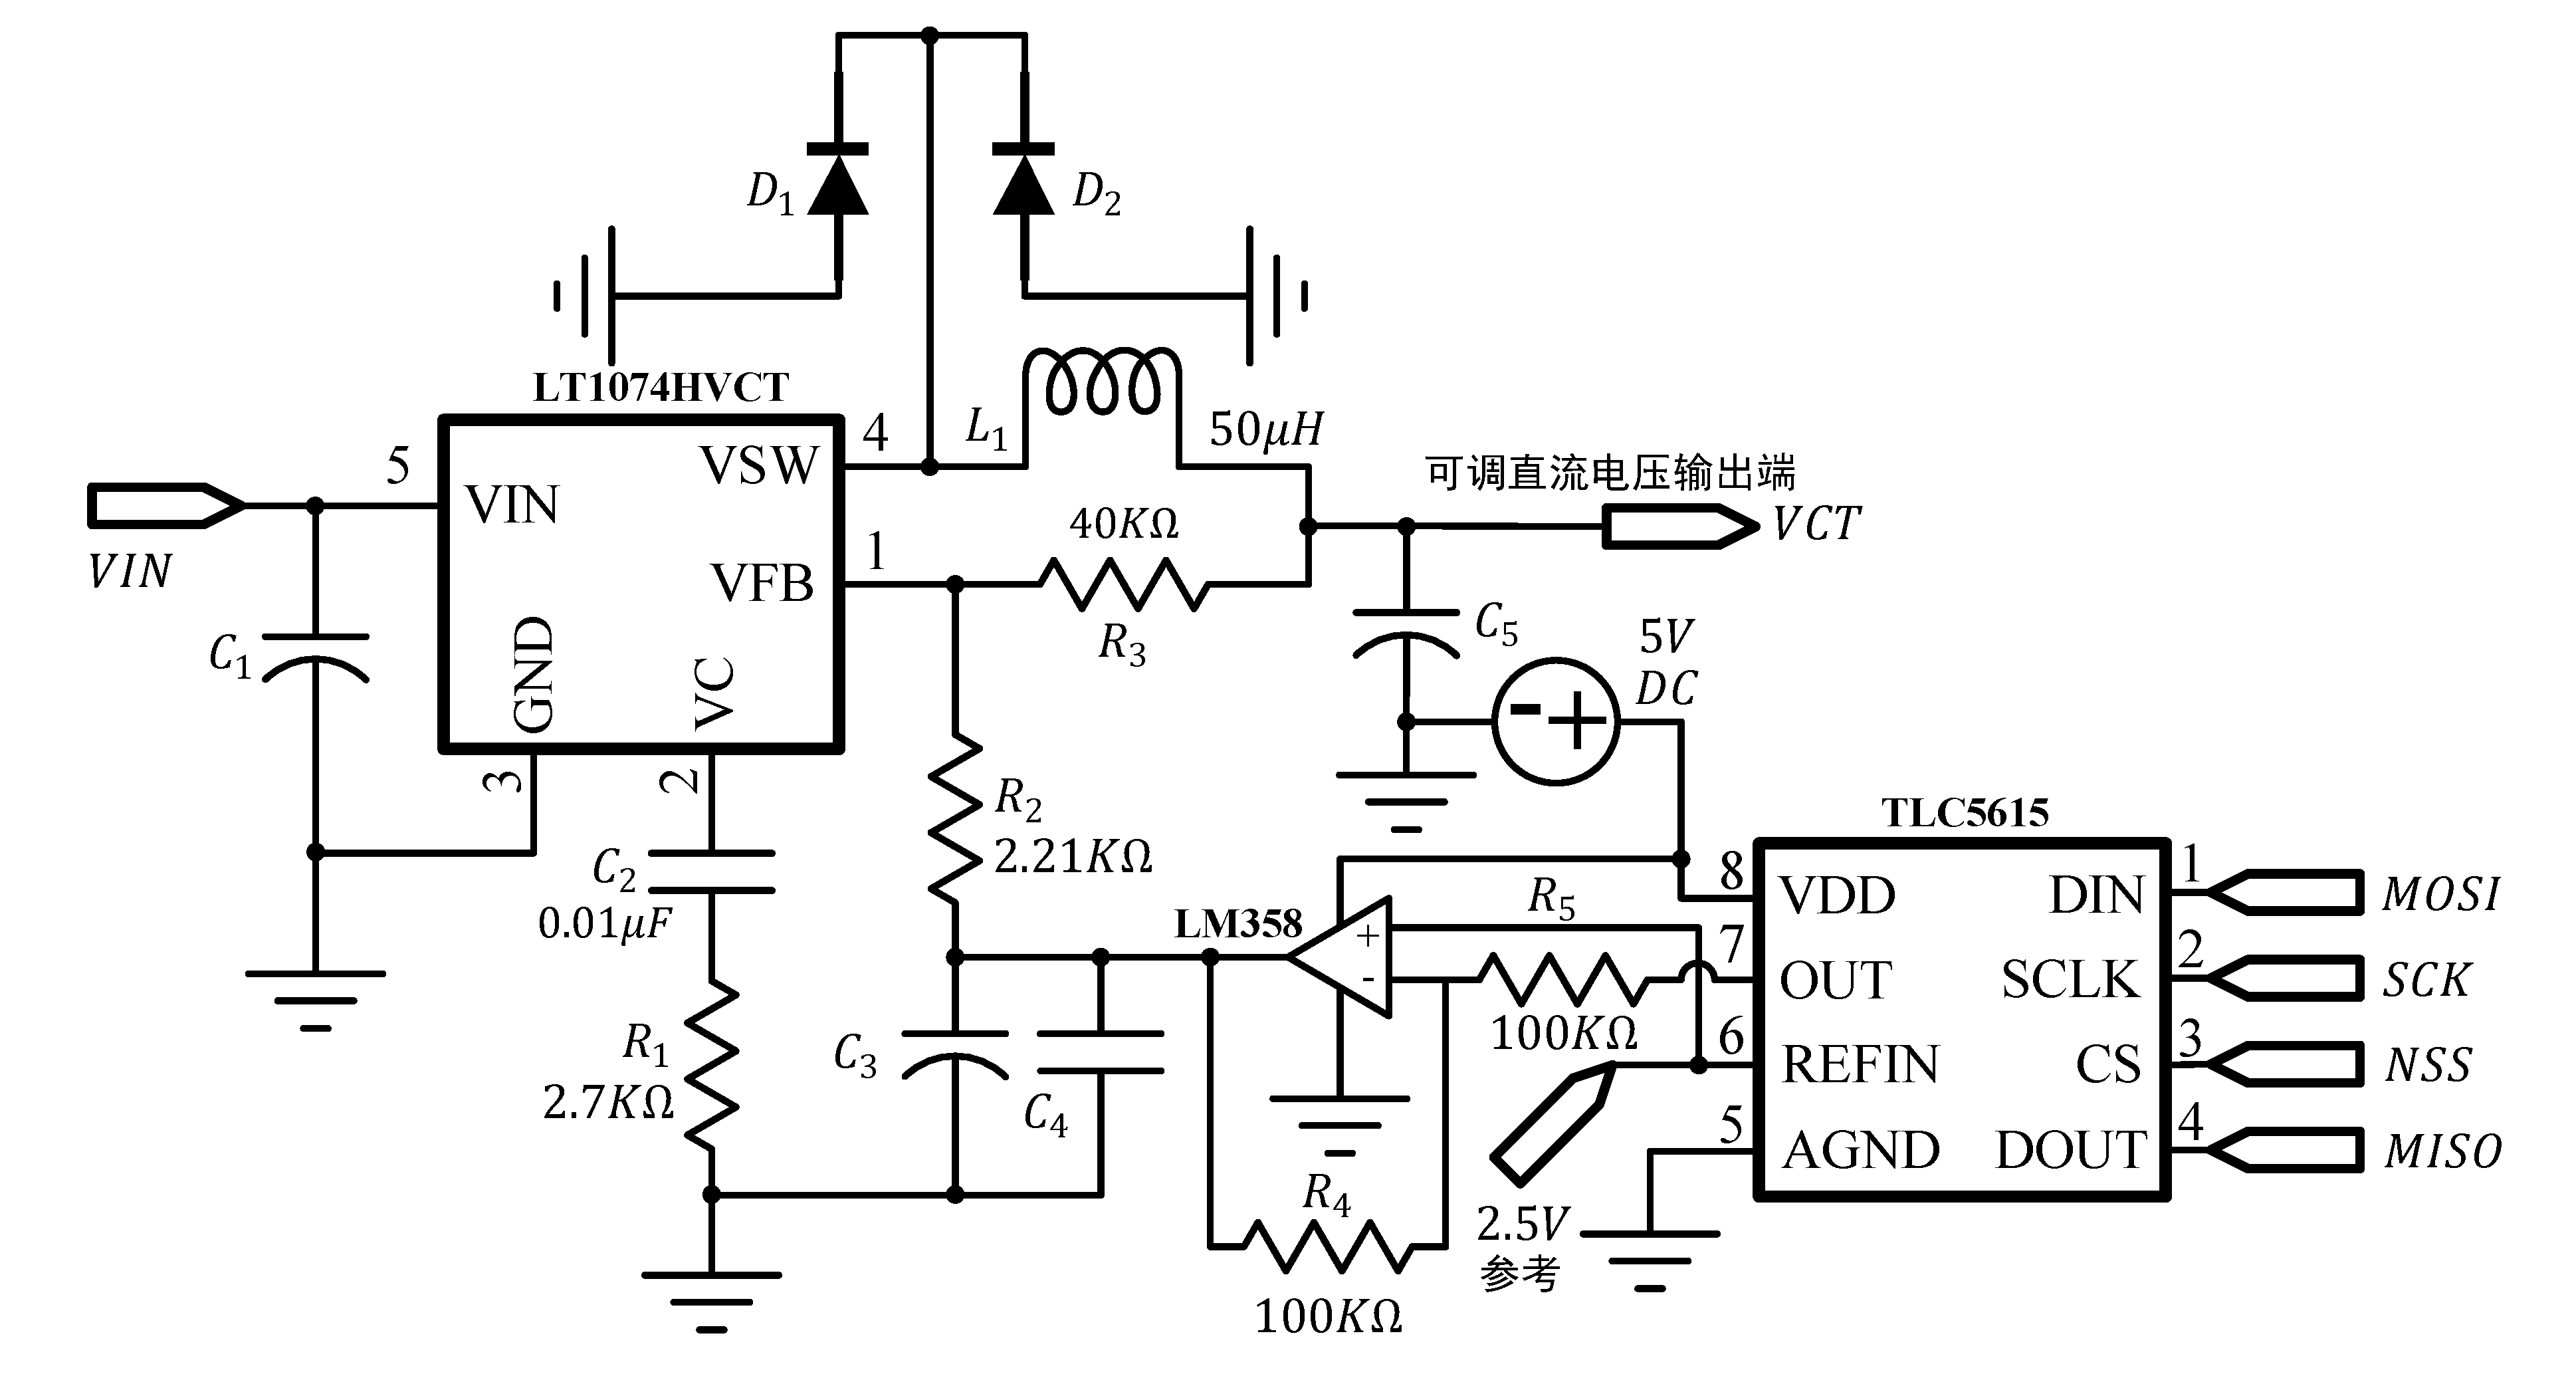
\includegraphics[scale=0.259]{Fig/buck_adjust.pdf}
\caption{\label{buck_adjust}可调直流稳压源电路}
\end{figure}

LT1074是一款高压高电流 DC-DC 开关稳压器芯片，内部集成了功率开关管、驱动控制振荡器、误差放大器、反馈调节环路以及过流保护等模块。在输出电压调节工作过程中，芯片内部振荡器以 100 kHz 的固定开关频率驱动内部功率开关管进行周期性导通与关断，实现对输入电压的脉宽调制（PWM）控制。当输出电压升高时，经分压电阻$R_2$、$R_3$形成的反馈电压VFB随之上升并高于芯片内部2.21V的基准参考电压，则误差放大器检测到正向偏差，并通过内部补偿与振荡控制环节减小开关管驱动信号的占空比，从而单位周期内传递至负载的能量降低，输出电压下降并恢复至稳态值。当输出电压降低时反之，该负反馈调节机制保证了稳压芯片在输入电压波动或负载变化条件下仍然能维持输出电压的稳定。在稳态工作条件下，输出电压和偏置电压满足关系式如下：
\begin{equation}
\frac{V_{VCT}-V_{VFB}}{R_3} = \frac{V_{VFB}-V_{C_3}}{R_2}
\end{equation}
式中，$V_{VCT}$为可调直流源输出电压，$V_{VFB}$为稳压器芯片反馈端输入电压，$V_{C_3}$为系统引入的偏置电压。为实现对偏置电压的数字化调节，本文采用数模转换器（DAC）结合运算放大器构成偏置电压数字控制电路。TLC5615是一款10位串行输入、电压输出型DAC芯片，其输入为二进制数字信号，输出为与输入数字量成比例的线性模拟电压。芯片输出电压范围为0～$V_{REF}$ 的两倍，其中参考电压由基准源芯片LM336Z提供2.5V稳定基准。非隔离区主控单元通过串行外设接口SPI（Serial Peripheral Interface Bus）向TLC5615发送待转换的数字量，DAC输出相应的模拟电压信号。为满足偏置电压极性及调节方向的要求，本文采用LM358双运算放大器中的一个运放单元构成反相放大器电路，对 DAC 输出电压进行极性变换与比例调整，使数字控制量的变化方向与可调直流稳压源输出电压的调节方向保持一致，从而保证系统控制逻辑的单调性与可预测性。

偏置电压调节过程中，由于LT1074内部使用的基准电压为2.21V，$V_{C_3}$处的偏置电压需满足0-2.21V的电压范围才能正常工作。根据图\ref{buck_adjust}所示的运算放大器电路，TLC5615的输出电压$V_{OUT}$与偏置电压满足如下关系式：
\begin{equation}
V_{C_3} = \frac{R_4}{R_5}(2.5V-V_{OUT})+2.5V = 5V - V_{OUT}  \label{eq_1}
\end{equation}

由数模转换芯片DAC的工作原理可知，TLC5615的输出电压$V_{OUT}$与输入的数字信号$D_{IN}$满足如下关系式：
\begin{equation}
V_{OUT} = 2V_{REF}\times\frac{D_{IN}}{2^{10}} = 5V \times \frac{D_{IN}}{1024}  \label{eq_2}
\end{equation}
其中，$V_{REF}$为DAC的参考电压，且TLC5615芯片的内部增益设定为2。根据前文分析可知，偏置电压满足$V_{C_3} < 2.21V$，将条件代入式(\ref{eq_1})可得输出电压满足$V_{OUT} > 2.79V$，进一步结合式(\ref{eq_2})可推得，非隔离区MCU输入的数字信号$D_{IN}$的有效取值范围为$571 < D_{IN} < 1024$，当数字输入信号增加至最大值时，DAC输出电压相应提高，使可调直流稳压源的偏置电压趋近于0，此时稳压器输出电压达到最大值。

综上所述，通过改变输入数字控制量$D_{IN}$，可以改变稳压器的反馈偏置电压，最终实现对馈入推挽逆逆变电路的可调直流母线电压的调节。由于推挽逆变器输出功率与其输入直流母线电压幅值密切相关，因此该控制方式实现了对高频信号输出功率的连续可调控制。

\subsection{推挽逆变电路}
\subsubsection{核心芯片选型}
推挽逆变电路中使用到的核心器件是功率开关器件及其驱动芯片，常用的开关器件有MOSFET和IGBT两种。MOSFET具有开关速度快、驱动简单、导通压降低等优点，但耐压和抗辐射能力较差，适合中小功率与高频率工作场合；IGBT具有耐压高、抗辐射能力强等优点，适合大功率应用场景，但开关速度较慢，驱动电路复杂，导通压降较高。由于本系统所设计的架构中前级可调直流电压源输出范围较小，且开关频率为高频350KHz，因此使用MOSFET作为功率开关器件，并相应地选取合适的MOSFET驱动芯片，芯片的选型将直接影响高频刀手术系统输出信号的质量，本节将详细介绍这两种芯片的选型。

结合推挽逆变电路的拓扑结构，前级可调直流电压源从变压器初级线圈的中心抽头输入，当单个MOSFET导通期间，变压器初级线圈的另一半将会电磁感应产生与输入直流电压源大小相同的感应电压叠加在漏源两端，因此单个MOSFET的耐压值最小应为输入电压源的两倍。本文设计的可调直流电压源输出电压范围为2.5V-48V，因此MOSFET的耐压值应不小于96V。考虑到实际应用中可能出现的电压尖峰等问题，选择耐压值大于150V的MOSFET芯片作为功率开关器件。对于开关频率而言，由于系统输出信号频率为350KHz，开关周期为2857ns，推挽逆变电路中每个MOSFET导通半个周期，考虑到一定的驱动信号死区时间设置裕度，单个开关管导通时间至少为1329ns，因此所选开关器件的上升时间和下降时间必须远小于此值，才能保证正常的开通和关断。在开关器件损耗方面，选择导通电阻和门级电荷较小的MOSFET芯片以降低开关损耗和导通损耗，提高系统效率。综上所述经过综合选型，最终选择型号为IRF640N的MOSFET芯片作为功率开关器件，其主要工作参数如表\ref{IRF640N}所示。

\begin{table}[htbp]
    \caption{\label{IRF640N}IRF640N主要工作参数}
    \centering
    \small
    \setlength{\tabcolsep}{20pt}
	\begin{tabular}{c c c c }
        \hline
        参数 & 数值 & 参数 & 数值 \\
        \hline
        最大漏源电压  & 200V  & 漏源导通电阻 & 0.15$\Omega$ @10V\\
        最大栅源电压  & $\pm$20V & 门级电荷 & 67 nC \\
        最大连续漏源电流 & 18A @25℃    & 上升时间 & 19ns \\
        最大耗散功率 & 150W @25℃  & 下降时间 & 5.5ns \\
        \hline
    \end{tabular}
\end{table}


\subsection{高频信号放大模块}
\subsubsection{高频变压器}

\subsubsection{LC谐振网络}

\section{高频输出信号检测模块设计}

\subsection{输出电压信号检测}

\subsection{输出电流信号检测}

\section{人机交互模块设计}

\section{基于SPICE模型的仿真实验分析}

\section{本章小结}








